\section{Vorlesung 11: Andere Prozessbeschreibungssprachen}

In dieser Vorlesung betrachten wir UML-Aktivitätsdiagramme und Bezüge dieser Modellierungssprache zu Petrinetzen.

Aktivitätsdiagramme 
\marginline{Aktivitäts\-diagramme}
sind eigentlich geklaute Petrinetze mit einer anderen Syntax und ergänzenden Notationen, aber derselben Semantik. Wie Petrinetze kann man Aktivitätsdiagramme sowohl zur Modellierung von Prozessen als auch zur Modellierung von Abläufen einsetzen, allgemeinere Systeme sind dagegen nicht im Fokus von Aktivitätsdiagrammen. Man kann sie in unterschiedlichen Abstraktionsgraden und für unterschiedliche Zwecke in allen Kernprozessen des Softwareengineering verwenden. Sie sind extrem mächtig, da sie sehr viele unterschiedliche Notationselemente zur Verfügung stellen.

Während der Anforderungsermittlung 
\marginline{Einsatzbereiche}
in einem Softwareentwicklungsprojekt werden Aktivitätsdiagramme häufig zur Darstellung von Geschäftsprozessen der Real\-welt verwendet. Ein zweiter Einsatzbereich ist die differenziertere Modellierung von Abläufen der Anwendungsfälle aus einem UML-Anwendungsfalldiagramm (dieses lernen Sie in Lektion~4 kennen). Beides erfolgt stark Nutzersicht-zentriert, dafür wird in der Regel nur ein Bruchteil der zur Verfügung stehenden Notationselemente benötigt. Aber auch für den implementierungsnahen Einsatz bieten Aktivitäts\-diagramme viele Möglichkeiten. So lassen sich sowohl interne Systemprozesse als auch Algorithmen mit ihnen modellieren. Dafür kommen dann auch etwas komplexere Notationsmöglichkeiten des Diagrammtyps wie Schleifen, Zustandsvariablen oder Ausnahmebehandlungen zum Tragen.


\begin{figure}
	\centering
	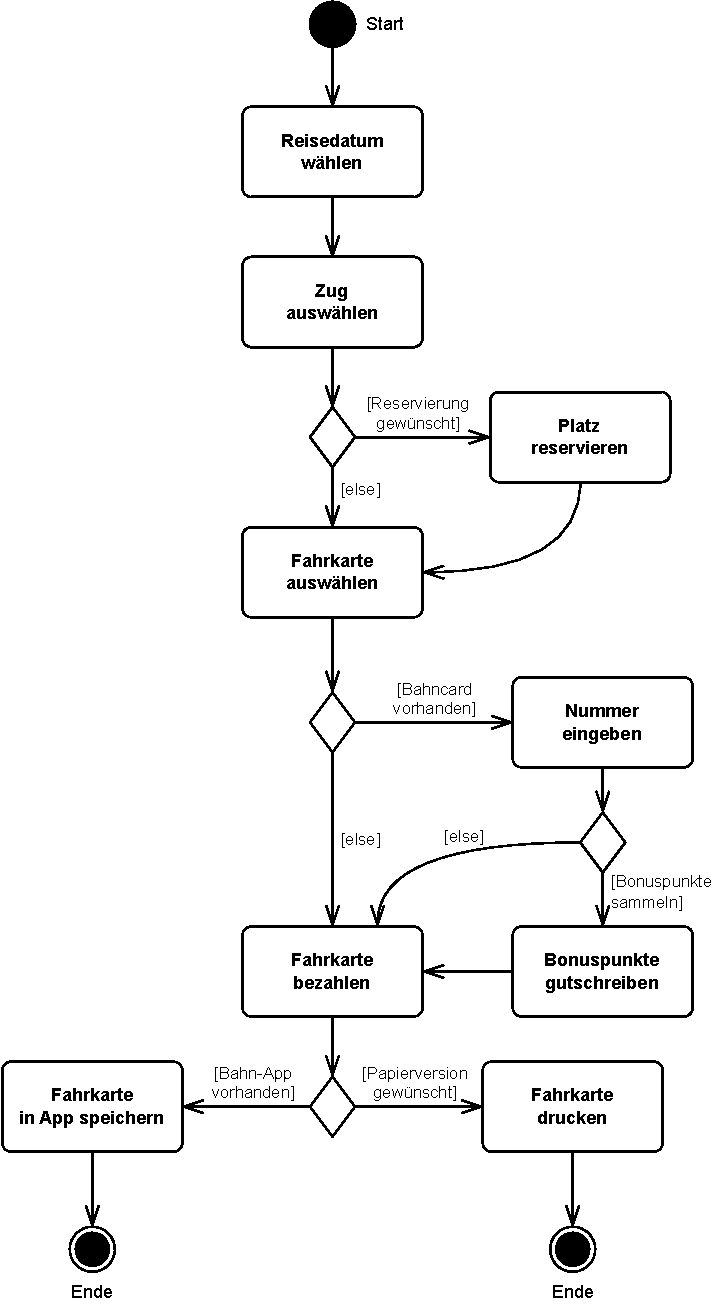
\includegraphics[scale=0.7]{Bilder/Kapitel-5/aktivitaetsdiagramm_fahrkarte_kaufen.pdf}
	\caption{Aktivitätsdiagramm für die Aktivität Fahrkartenkauf}
	\label{fig:aktivitaetsdiagramm_fahrkarte_kaufen}
\end{figure}

Abbildung~\ref{fig:aktivitaetsdiagramm_fahrkarte_kaufen} zeigt ein Aktivitätsdiagramm für eine \textit{Aktivität} Fahrkartenkauf. Vorsicht: das Aktivitätsdiagramm unterscheidet nicht sauber zwischen Prozessebene und Ablaufebene! Die Benennungen „Aktivität“ und „Aktion“ werden auf derselben Ebene verwendet, und sie bedeuten etwas anderes als bei uns. Auch wird nicht unterschieden, ob es um ein Prozessmodell oder um den modellierten Prozess geht. 

Als Aktivität wird der Prozess als Gesamtes bezeichnet, 
\marginline{Syntax und Semantik}
also hier die Aktivität "`Fahrkartenkauf"'. Die einzelnen \textit{Schritte} in dieser Aktivität sind die \textit{Aktionen}, wie „Reisedatum auswählen“ oder „Fahrkarte bezahlen“. Diese werden mit abgerundeten Rechtecken dargestellt. Die Pfeile repräsentieren den Kontrollfluss, die Ausführungsreihenfolge zwischen den Aktionen. Wie im Zustandsdiagramm ist der schwarz ausgemalte Kreis der Startknoten, der spezifiziert, bei welcher Aktion die Aktivität Fahrkartenkauf beginnt.

Die Rauten sind sogenannte \textit{Entscheidungsknoten}. Ein Entscheidungsknoten hat genau einen eingehenden Kontrollfluss und beliebig viele ausgehende, von denen bei einer konkreten Ausführung der Aktivität aber nur genau einer fortgeführt wird. Die ausgehenden Pfeile des Entscheidungsknotens sind mit Bedingungen (Guards) versehen, die wie bei höheren Petrinetzen und bei Zustandsdiagrammen in eckigen Klammern notiert werden. Auch hier die Parallele zu den Zustandsdiagrammen: die Guards eines Entscheidungsknotens müssen sich gegenseitig ausschließen und sollten alle Auswahlmöglichkeiten abdecken, so dass der weitere Kontrollfluss eindeutig festgelegt ist. Ein oder mehrere Endknoten (schwarzer Kreis mit weißer Umrandung) spezifizieren, nach welchen Aktionen eine Aktivität enden kann.

Analog zum Element \textit{Entscheidungsknoten} bietet das Aktivitätsdiagramm auch einen \textit{Verbindungsknoten} an, wenn Kontrollflüsse wieder zusammenlaufen. Dieser wird ebenfalls über eine Raute dargestellt. Er unterscheidet sich vom Entscheidungsknoten dadurch, dass beliebig viele Kontrollflüsse hereinführen, aber nur genau einer herausführt. Häufig lässt man Verbindungsknoten im Diagramm weg und führt die Kontrollflüsse direkt in der Aktion wieder zusammen -- so auch hier in der Abbildung. Die UML erlaubt es, in ähnlicher Weise auch auf die Entscheidungsknoten zu verzichten, aber das macht ein Aktivitätsdiagramm meistens unübersichtlicher. Zumindest bei Aktivitätsdiagrammen im Rahmen der Anforderungsermittlung sollte man Entscheidungsknoten daher nicht weglassen.


\begin{figure}[h!]
	\centering
	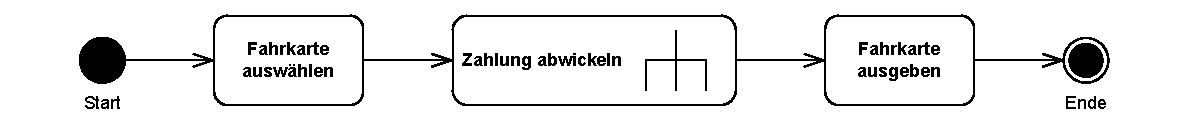
\includegraphics[scale=0.7]{Bilder/Kapitel-5/aktivitaetsaufruf_zahlung.pdf}
	\caption{Aktivitätsaufruf "`Zahlung abwickeln"'}
	\label{fig:aktivitaetsaufruf_zahlung}
\end{figure}

\begin{figure}[h!]
	\centering
	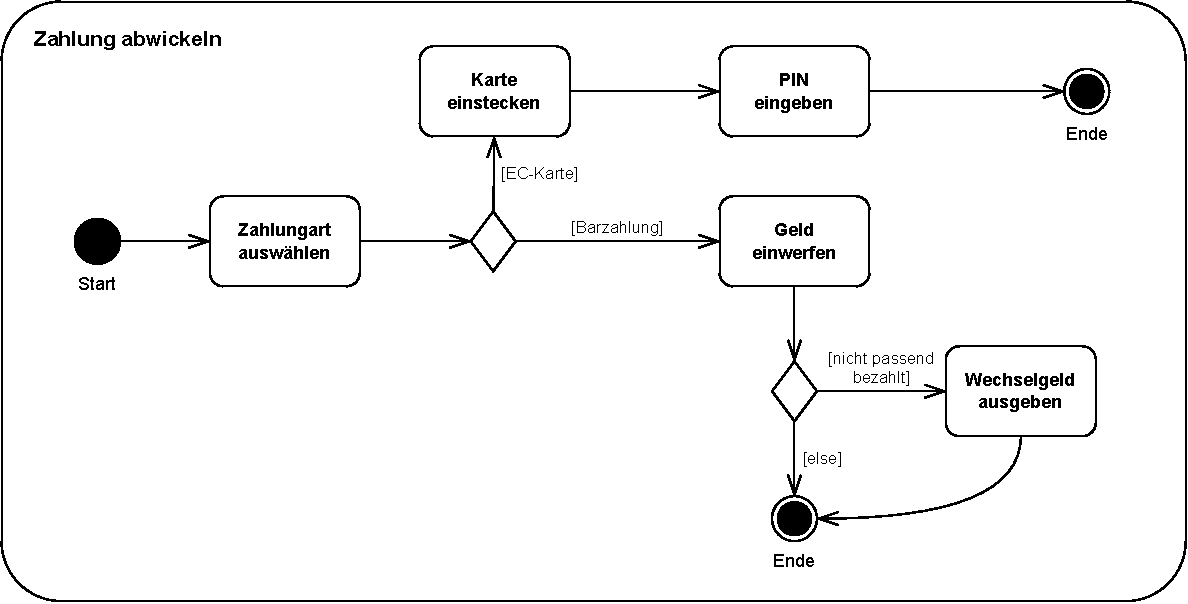
\includegraphics[scale=0.7]{Bilder/Kapitel-5/aktivitaetsdiagramm_zahlung_abwickeln.pdf}
	\caption{Aktivitätsdiagramm "`Zahlung abwickeln"'}
	\label{fig:aktivitaetsdiagramm_zahlung_abwickeln}
\end{figure}

Wenn Aktivitäten sehr kleinschrittig (viele einzelne Aktionen) beschrieben werden sollen, können Aktivitätsdiagramme schnell unübersichtlich werden. Oft bietet es sich an, ein Aktivitätsdiagramm auf einem hohen Abstraktionsniveau als Übersicht zu haben und dessen einzelne Aktionen in jeweils eigenen Diagrammen verfeinert zu modellieren. Abbildung~\ref{fig:aktivitaetsaufruf_zahlung} zeigt ein sehr übersichtliches Diagramm für eine Aktivität „Fahrkarte kaufen“ an einem Automaten. Bei der Aktion „Zahlung abwickeln“ in diesem Diagramm ist durch das Gabel-Symbol rechts im Kästchen gekennzeichnet, dass hier ein Aktivitätsaufruf erfolgt, und zwar der Aufruf der Aktivität „Zahlung abwickeln“, die in einem eigenen Aktivitätsdiagramm modelliert ist. Dieses ist in Abbildung~\ref{fig:aktivitaetsdiagramm_zahlung_abwickeln} dargestellt.
 
\pagebreak %%% für Druck

Im Rahmen der Domänenmodellierung werden Aktivitätsdiagramme vor allem zur Modellierung von Geschäftsprozessen der Domäne eingesetzt. Häufig geht es dabei auch darum herauszufinden, welche Akteure in welcher Art und Weise am Geschäftsprozess beteiligt sind, also wer welche Tätigkeiten im Rahmen des Geschäfts\-prozesses ausführt. Das UML-Aktivitätsdiagramm bietet das Element \textit{Aktivitäts\-bereich} an, um die Verantwortung für Aktionen bestimmten Akteuren zuzuordnen. Dies ist ein ähnliches Konzept wie Pools und Lanes in BPMN. Abbildung~\ref{fig:aktivitaetsdiagramm_futterannahme} zeigt ein Diagramm mit drei Aktivitätsbereichen für die Akteure „Tierpfleger“, „Lager\-verwalter“ und „Zooverwaltung“ für eine Aktivität „Futterannahme“. Durch die Platzierung in den Aktivitätsbereichen ist deutlich, wer welche Aktionen ausführt.
  

\begin{figure}[h!]
	\centering
	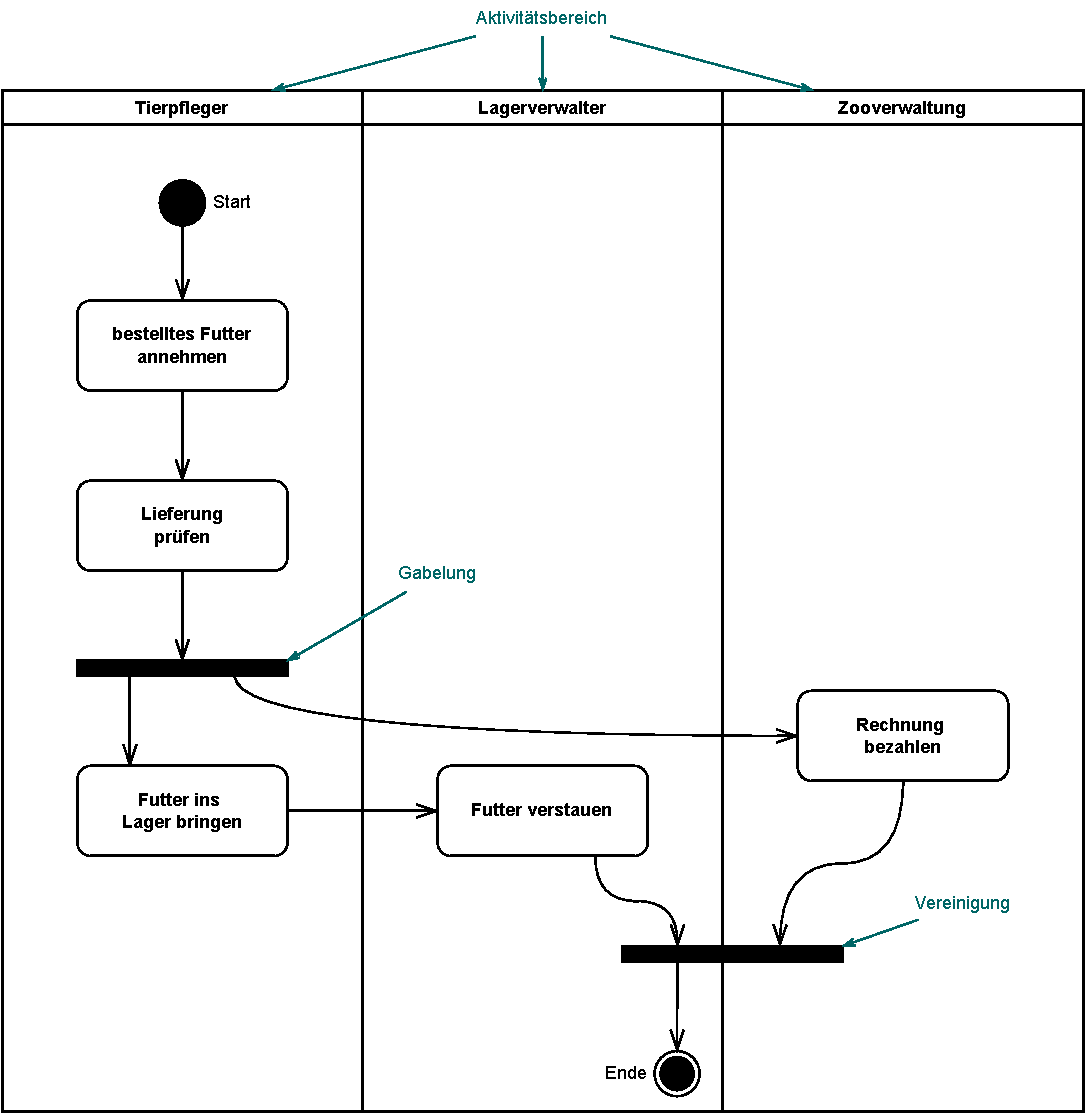
\includegraphics[scale=0.7]{Bilder/Kapitel-5/aktivitaetsdiagramm_futterannahme.pdf}
	\caption{Aktivitätsdiagramm Futterannahme}
	\label{fig:aktivitaetsdiagramm_futterannahme}
\end{figure}

Abbildung~\ref{fig:aktivitaetsdiagramm_futterannahme} zeigt außer den Aktivitätsbereichen auch die Elemente für die Model\-lie\-rung
sogenannter \textit{Gabelungen} (oberer schwarzer Balken). Diese sind unabhängig von den Aktivitätsbereichen, hätten also auch in den vorherigen Diagrammen verwendet werden können. Die Gabelung teilt einen Kontrollfluss in mehrere Kontrollflüsse auf, die nebenläufig laufen. Das Pendant, um die Nebenläufigkeit wieder zu beenden, ist die sogenannte \textit{Vereinigung}, die Sie rechts unten im Diagramm sehen. Die Vereinigung fasst mehrere Kontrollflüsse zu einem Kontrollfluss zusammen. Hier in der Abbildung modelliert sie, dass sowohl die Aktion „Futter verstauen“ vom Akteur „Lagerverwalter“ als auch die Aktion „Rechnung bezahlen“ vom Akteur „Zooverwaltung“ abgeschlossen sein müssen, bevor die Aktivität „Futterannahme“ beendet ist. Dieses Beispiel erinnert eher an einen halbgeordneten Petrinetz-Ablauf.

Sicherlich sind Ihnen die Ähnlichkeiten zwischen Aktivitätsdiagrammen und Petri\-netzen bereits aufgefallen. Die folgende Tabelle zeigt nochmal eine Gegenüber\-stellung verschiedener Elemente in der Syntax der beiden Prozess\-beschreibungs\-sprachen. In der Vorlesung werden zusätzlich die Ähnlichkeiten der Petrinetze zu den aus Vor\-lesung~1 bekannten Geschäftsprozess-Modellierungssprachen EPK und BPMN aufgezeigt.


\begingroup
	\setlength{\tabcolsep}{10pt} % Default value: 6pt
	\renewcommand{\arraystretch}{1.5} % Default value: 1
	
	% Hilfsvariablen
	\newcommand{\sttpHilfA}{0.25\textwidth} % Breite der linken Spalte	(Beschreibung)
	\newcommand{\sttpHilfB}{0.25\textwidth} % Breite der der mittleren und der rechten Spalte(Abbildungen)
	\newcommand{\sttpFaktor}{0.8} % Skalierungsfaktor für die Grafiken
	\newcommand{\sttpAbstandRand}{5mm}
	
	% Die einzelnen Grafiken wurden mit einer Rahmenbreite von "0" in DrawIO exportiert.
	
	%\begin{figure}[!htbp]
	%	\centering
	\begin{longtable}{p{\sttpHilfA}|c|c}

		% \hline %-----------------------------

			\parbox{\sttpHilfA}{\centering
				\textbf{Element}} 
		&
			\textbf{Aktivitätsdiagramm} 
		&
			\textbf{Petrinetze} 
		\\
			
		\hline %-----------------------------
		\hline %-----------------------------
		\endhead
		
			\parbox{\sttpHilfA}{\centering
				Aktivität}
		&
			\parbox{\sttpHilfB}{\centering
				\vspace{\sttpAbstandRand}
				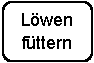
\includegraphics[scale=\sttpFaktor]{Bilder/Kapitel-5/gegenueberstellung_1a.pdf}
				\vspace{\sttpAbstandRand}
			} 
		&
			\parbox{\sttpHilfB}{\centering
				\vspace{\sttpAbstandRand}
				
\includegraphics[scale=\sttpFaktor]{Bilder/Kapitel-5/gegenueberstellung_1b.pdf}
				\vspace{\sttpAbstandRand}
			} 
		\\
		
		\hline %-----------------------------
		
			\parbox{\sttpHilfA}{\centering
				Vor- und \\ Nachbedingung} 
		& 
			\parbox{\sttpHilfB}{\centering
				\vspace{\sttpAbstandRand}
				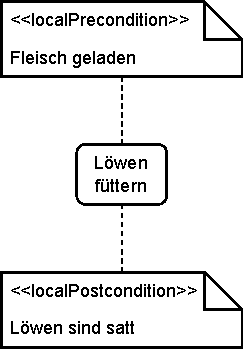
\includegraphics[scale=\sttpFaktor]{Bilder/Kapitel-5/gegenueberstellung_2a.pdf}
				\vspace{\sttpAbstandRand}
			} 
		&
			\parbox{\sttpHilfB}{\centering
				\vspace{\sttpAbstandRand}
				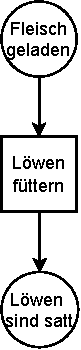
\includegraphics[scale=\sttpFaktor]{Bilder/Kapitel-5/gegenueberstellung_2b.pdf}
				\vspace{\sttpAbstandRand}
			} 
		\\
	
		\hline %-----------------------------
	
			\parbox{\sttpHilfA}{\centering
				Kontrollfluss}
		&  
			\parbox{\sttpHilfB}{\centering
				\vspace{\sttpAbstandRand}
				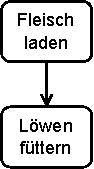
\includegraphics[scale=\sttpFaktor]{Bilder/Kapitel-5/gegenueberstellung_3a.pdf}
				\vspace{\sttpAbstandRand}
			}
		& 
			\parbox{\sttpHilfB}{\centering
				\vspace{\sttpAbstandRand}
				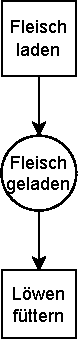
\includegraphics[scale=\sttpFaktor]{Bilder/Kapitel-5/gegenueberstellung_3b.pdf}
				\vspace{\sttpAbstandRand}
			}
		\\
		
		\hline %-----------------------------
		
			\parbox{\sttpHilfA}{\centering
				Aktivitätsbereich \\ / \\ Komponente} 
		& 
			\parbox{\sttpHilfB}{\centering
				\vspace{\sttpAbstandRand}
				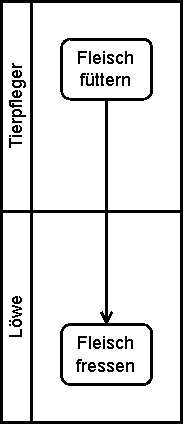
\includegraphics[scale=\sttpFaktor]{Bilder/Kapitel-5/gegenueberstellung_4a.pdf}
				\vspace{\sttpAbstandRand}
			} 
		& 
			\parbox{\sttpHilfB}{\centering
				\vspace{\sttpAbstandRand}
				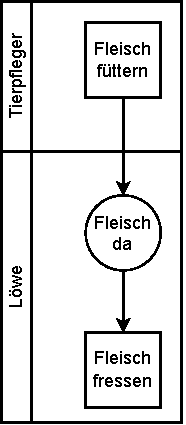
\includegraphics[scale=\sttpFaktor]{Bilder/Kapitel-5/gegenueberstellung_4b.pdf}
				\vspace{\sttpAbstandRand}
			} 
		\\
		
		\hline %-----------------------------
		
			\parbox{\sttpHilfA}{\centering
				Objektknoten \\ / \\ Marken und \\ Kantengewichte} 
		& 
			\parbox{\sttpHilfB}{\centering
				\vspace{\sttpAbstandRand}
				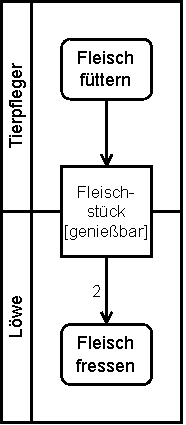
\includegraphics[scale=\sttpFaktor]{Bilder/Kapitel-5/gegenueberstellung_5a.pdf}
				\vspace{\sttpAbstandRand}
			}
		& 
			\parbox{\sttpHilfB}{\centering
				\vspace{\sttpAbstandRand}
				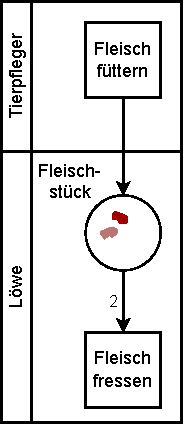
\includegraphics[scale=\sttpFaktor]{Bilder/Kapitel-5/gegenueberstellung_5b.pdf}
				\vspace{\sttpAbstandRand}
			} 
		\\

		\hline %-----------------------------

			\parbox{\sttpHilfA}{\centering
				Anfang \\ und \\ Ende } 
		&  
			\parbox{\sttpHilfB}{\centering
				\vspace{\sttpAbstandRand}
				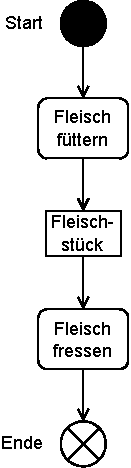
\includegraphics[scale=\sttpFaktor]{Bilder/Kapitel-5/gegenueberstellung_6a.pdf}
				\vspace{\sttpAbstandRand}
			}
		& 
			\parbox{\sttpHilfB}{\centering
				\vspace{\sttpAbstandRand}
				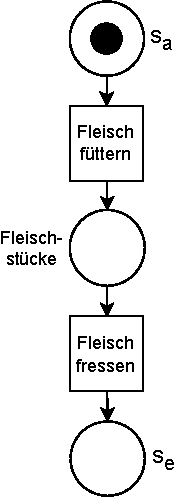
\includegraphics[scale=\sttpFaktor]{Bilder/Kapitel-5/gegenueberstellung_6b.pdf}
				\vspace{\sttpAbstandRand}
			} 
		\\
		
		\hline %-----------------------------
		
			\parbox{\sttpHilfA}{\centering
				Entscheidungs\-knoten} 
		&  
			\parbox{\sttpHilfB}{\centering
				\vspace{\sttpAbstandRand}
				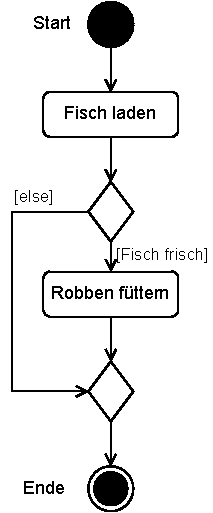
\includegraphics[scale=\sttpFaktor]{Bilder/Kapitel-5/gegenueberstellung_7a.pdf}
				\vspace{\sttpAbstandRand}
			} 
		& 
			\parbox{\sttpHilfB}{\centering
				\vspace{\sttpAbstandRand}
				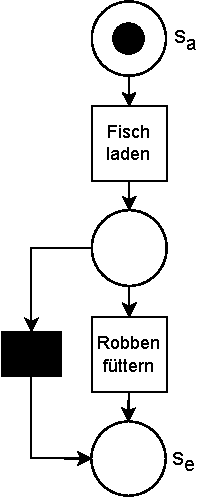
\includegraphics[scale=\sttpFaktor]{Bilder/Kapitel-5/gegenueberstellung_7b.pdf}
				\vspace{\sttpAbstandRand}
			} 
		\\
		
		\hline %-----------------------------
	\end{longtable}
	%	\caption{Gegenüberstellung von Aktivitätsdiagramm- und Petrinetz-Syntax}
	%	\label{fig:gegenueberstellung}
	%\end{figure}

\endgroup
